\subsection{SPIQA (Scientific Paper Image Question Answering)}
{{\footnotesize
\noindent SPIQA assesses AI models' ability to interpret and answer questions about figures
and tables in scientific papers by integrating visual and textual modalities 
with chain-of-thought reasoning.


\begin{description}[labelwidth=4cm, labelsep=1em, leftmargin=4cm, itemsep=0.1em, parsep=0em]
  \item[date:] 2024-07-12
  \item[version:] 1
  \item[last\_updated:] 2024-07-12
  \item[expired:] false
  \item[valid:] yes
  \item[valid\_date:] 2024-07-12
  \item[url:] \href{https://arxiv.org/abs/2407.09413}{https://arxiv.org/abs/2407.09413}
  \item[doi:] 10.48550/arXiv.2407.09413
  \item[domain:] Computer Science
  \item[focus:] Multimodal QA on scientific figures
  \item[keywords:]
    - multimodal QA
    - figure understanding
    - table comprehension
    - chain-of-thought
  \item[licensing:] Apache 2.0 License
  \item[task\_types:]
    - Question answering
    - Multimodal QA
    - Chain-of-Thought evaluation
  \item[ai\_capability\_measured:]
    - Visual-textual reasoning in scientific contexts
  \item[metrics:]
    - Accuracy
    - F1 score
  \item[models:]
    - Chain-of-Thought models
    - Multimodal QA systems
  \item[ml\_motif:]
    - Scientific paper reading
  \item[type:] Benchmark
  \item[ml\_task:]
    - Supervised Learning
  \item[solutions:] 0
  \item[notes:] Good
  \item[contact.name:] Subhashini Venugopalan
  \item[contact.email:] vsubhashini@google.com
  \item[datasets.links.name:] Hugging Face
  \item[datasets.links.url:] \href{https://huggingface.co/datasets/google/spiqa}{https://huggingface.co/datasets/google/spiqa}
  \item[results.links.name:] unknown
  \item[results.links.url:] \href{unknown}{unknown}
  \item[fair.reproducible:] True
  \item[fair.benchmark\_ready:] True
  \item[id:] spiqa\_scientific\_paper\_image\_question\_answering
  \item[Citations:] \cite{zhong2024spiqa}
\end{description}

{\bf Ratings:} ~ \\

\begin{tabular}{p{0.15\textwidth} p{0.07\textwidth} p{0.7\textwidth}}
\hline
Rating & Value & Reason \\
\hline
dataset & 4.5 & Dataset is available (via paper/appendix), includes train/test/valid split. FAIR-compliant with minor gaps in versioning or access standardization.
 \\
documentation & 5 & All information provided in paper
 \\
metrics & 5 & Uses quantitative metrics (Accuracy, F1) aligned with the task
 \\
reference\_solution & 2 & Multiple model results (e.g., GPT-4V, Gemini) reported; baselines exist, but full runnable code not confirmed for all.
 \\
software & 0 & Not provided
 \\
specification & 5 & Task administration clearly defined; prompt instructions explicitly given, no ambiguity in format or scope.
 \\
\hline
\end{tabular}

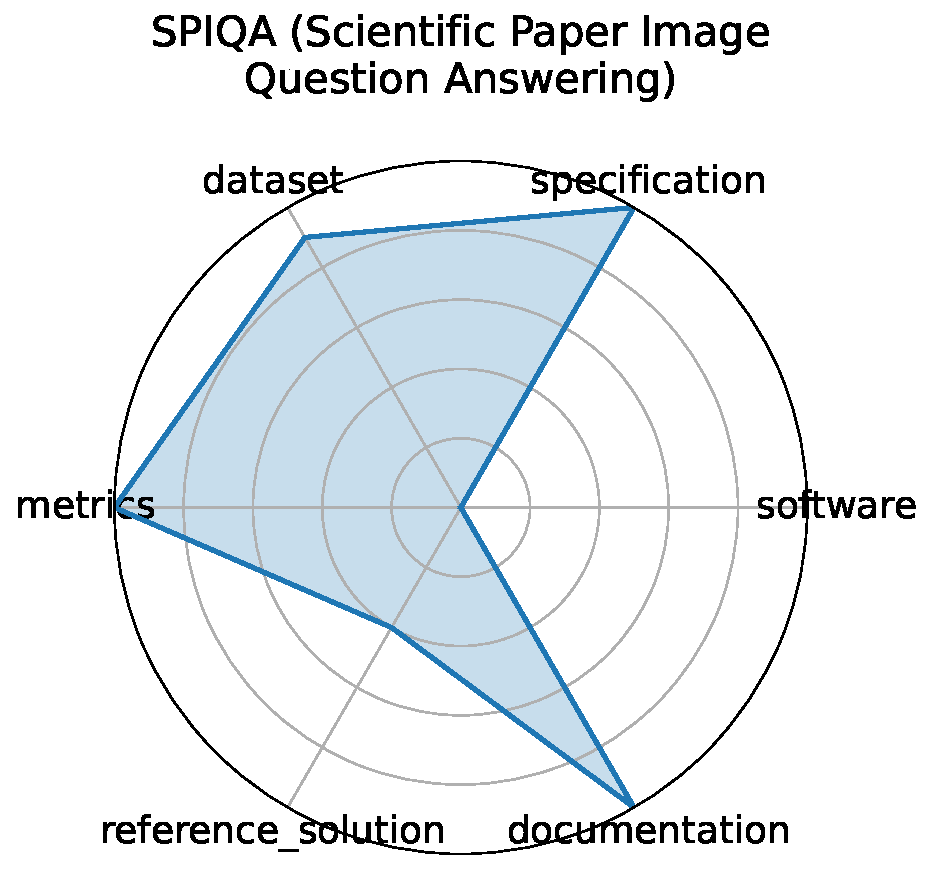
\includegraphics[width=0.2\textwidth]{spiqa_scientific_paper_image_question_answering_radar.pdf}
}}
\clearpage